\chapter{Käytännön toteutus\label{example}}

Tutkielmassa on nyt käsitelty DevOps-toimintamallia ja sen yhteydessä käytettäviä julkaisutapoja ja orkestrointiratkaisuja.
Osana tutkielmaa esitetään käytännön toteutus käsiteltyjen aiheiden käytöstä ohjelmistotuotannossa.
Helsingin Yliopiston Norppa-palautejärjes\-telmän kehitys perustuu DevOps-toimintamalliin ja palvelu käyttää monia tutkielmassa käsiteltyjä teknologioita.

Palvelun perustoiminta ja ohjelmistoarkitehtuuri esitetään tässä luvussa.
Olen osallistunut järjestelmän ohjelmistotuotantoon Toskassa ja toteuttanut tässä luvussa esitettävän OpenShift-pohjaisen konttiorkestrointiratkaisun.

\section{Norppa-palautejäjestelmä}

Helsingin yliopiston tietojenkäsittelytieteen osaston sovelluskehitysakatemian (\textit{Toska}) \cite{Tenhunen23} kehittämä kurssipalautejärjestelmä Norppa on tutkielmassa esitetyn DevOps-toimintamal\-lin mukaisessa aktiivisessa kehityksessä.
Järjestelmää käytetään Helsingin yliopiston lisäksi myös Tampereen yliopiston kurssipalautejärjestelmänä \cite{Tampere23}.

Norppa on integroitu Sisu-opintotietojärjestelmän \cite{Laukka20} kanssa.
Järjestelmä luo automaattisesti muokattavan palautelomakkeen ja tiedottaa Sisussa luodun kurssin opiskelijoille palautteen aukeamisesta.
Annetusta palautteesta luodaan yhteenveto, joka näytetään kurssin opiskelijoille ja opettajille.
Norppa tukee myös muun muassa avointa tekstuaalista jatkuvaa palautetta ja koulutusohjelma- sekä yliopistotason palautteen yhteenvetonäkymiä.

Järjestelmän on kehittänyt Helsingin Yliopiston Toska-tiimi, mutta jatkokehitystä tehdään yhteistyössä Tampereen yliopiston kanssa.
Kehitys perustuu avoimeen lähdekoodin ja DevOps-toimintamalliin.
Seuraavaksi esitellään Norpan kehityksessä ja tuotantokäytössä käytetyt tutkielman kannalta merkitykselliset ratkaisut.

\section{DevOps-toimintamallin käyttö}

Norppa on avoimen lähdekoodin projekti, jonka lähdekoodi ja versiohistoria säilötään GitHub-alustalla.
DevOps-toimintamallin mukainen jatkuva integraatio ja toimitus toteutetaan osana versiohallintaa \textit{GitHub Actions}-palvelun avulla.
Kaikissa toimintamallin vaiheissa käytetään konttiteknologiaa ja orkestrointiratkaisuna toimii Kubernetekseen perustuva OpenShift-konttiorkestrointialusta.

Kuva \ref{fig:norppa:deployment} esittää Norpan julkaisuputken ja käytetyt analytiikkapalvelut.
Kehittäjän viedessä uuden koodimuutoksen versiohallintaan uudesta koodiversiosta rakennetaan automaattisesti kontti, jota vasten suoritetaan testit.
Testauksen onnistuessa sama kontti viedään \textit{Quay.io}-konttirekisteriin, josta se haetaan julkaistavaksi testiympäristöön.
Uuden koodimuutoksen vieminen tuotantoympäristöön vaatii manuaalisen hyväksynnän, jonka seurauksena sama prosessi toistetaan, mutta julkaistu kontti merkitään vietäväksi tuotantoympäristöön.

\begin{figure}[ht]
\begin{center}
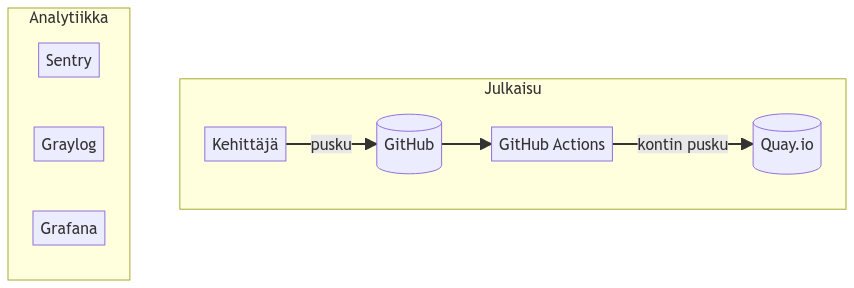
\includegraphics[width=1\textwidth]{figures/norppa_deployment.png}
\caption{Norpan julkaisuputki ja analytiikkapalvelut \cite{Norppa23}\label{fig:norppa:deployment}.}
\end{center}
\end{figure}

Koko julkaisuputki kestää noin 15 minuuttia ja mahdollistaa näin useat päivittäiset julkaisut.
Uusia toiminnallisuuksia tuodaan käyttöön osittain pienten yksittäisten julkaisujen kautta, jonka seurauksena koodimuutoksista saadaan nopeaa palautetta ja mahdollisiin ongelmiin voidaan reagoida nopeasti.

\section{Konttien orkestroinnin käyttö}

Norpan testi- ja tuotantoympäristönä toimii Helsingin yliopiston OpenShift-konttiorkes\-trointialusta \cite{Helsinki21}.
OpenShift on Kubernetekseen perustuva konttiorkestrointialusta, joka tarjoaa konttien orkestroinnin lisäksi muun muassa käyttäjähallinnan ja oman graaffisen käyttöliittymänsä~\cite{Lossent17}.
Kuvassa \ref{fig:norppa:deployment} esitetty julkaisuputki ja erillisellä virtuaalikoneella toimivat analytiikkapalvelut sijaitsevat OpenShift-klusterin ulkopuolella.

Kuva \ref{fig:norppa:architecture} esittää Norpan ohjelmistoarkkitehtuurin osana OpenShift-klusteria.
Saman ohjelmistoarkkitehtuurin mukaiset palvelut on toteutettu sekä testi- että tuotantoklustereissa.
Norppa koostuu ydinpalvelusta ja siihen liitettävistä erillisistä mikropalveluista.
Tämä arkkitehtuuriratkaisu mahdollistaa palvelun muokattavuuden.
Helsingin ja Tampereen yliopistot käyttävät samaa Norpan ydintä, mutta muut palvelut on toteutettu erikseen yliopistojen tarpeiden mukaisesti.

\begin{figure}[ht]
\begin{center}
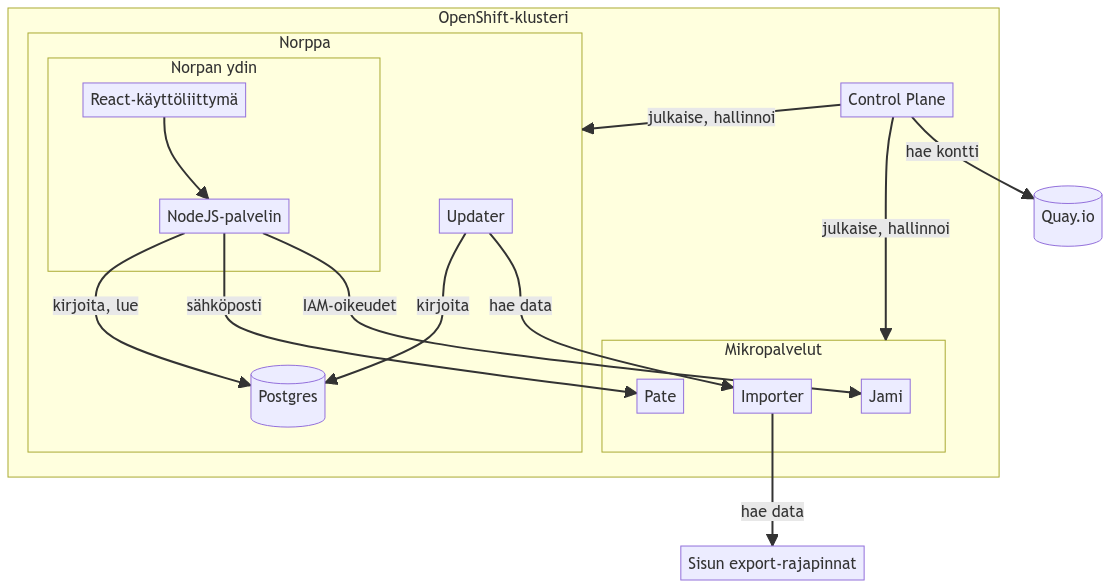
\includegraphics[width=1\textwidth]{figures/norppa_architecture.png}
\caption{Norpan laajennettu arkkitehtuuridiagrammi \cite{Norppa23}\label{fig:norppa:architecture}.}
\end{center}
\end{figure}

Norpan ydin muodostuu React pohjaisesta käyttöliittymästä ja NodeJS-palvelimesta.
Sisusta haetun opintodatan synkronisoinnista huolehtii erillinen Updater-palvelu.
Tämän lisäksi Norppa käyttää useita myös muiden järjestelmien käyttämiä mikropalveluita, kuten sähköpostipalvelua Pate ja käyttöoikeushallintapalvelua Jami.

Kaikki palvelut sijaitsevat samassa OpenShift-klusterissa, joka mahdollistaa helpon palveluiden välisen kommunikaation.
OpenShift-klusteri hakee \textit{Quay.io}-konttirekisteristä uuden kontin julkaisun yhteydessä ja huolehtii käytössä olevien konttien päivityksestä.
Julkaisujen lisäksi klusteri huolehtii luvun \ref{platforms} mukaisesti muun muassa resurssien käyttörajojen hallinnasta ja automaattisesta skaalautumisesta.

Ennen OpenShift-pohjaista konttiorkestrointiratkaisua Norppa ja sen käyttämät mikropalvelut oli toteutettu Helsingin yliopiston tietojenkäsittelytieteen osaston virtuaalikoneilla.
Järjestelmä käytti jo tässä vaiheessa virtuaalikoneiden lisäksi konttiteknologiaa, joka mahdollisti DevOps-toimintamallin mukaisen ohjelmistotuotannon.
Konttien orkestroinnin käyttöönotto kuitenkin yksinkertaisti muun muassa uusien ohjelmistoversioiden julkaisua ja paransi järjestelmän käytettävyysaikaa konttien orkestroinnin tarjoaman vikasietoisuuden vuoksi.

Norpan sekä Toskan muiden järjestelmien keskittäminen OpenShift-klusteriin mahdollisti 14 erikseen hallinnoitavan virtuaalikoneen sulkemisen.
Erilliset virtuaalikoneet vaativat ajoittain manuaalista hallinnointia muun muassa käyttöjärjestelmäpäivitysten ja tallennustilan hallinnan suhteen, joten ohjelmistoinfrastruktuurin ylläpitotaakka on vähentynyt.
Myös koko ohjelmistoinfrastruktuurin vakaus on lisääntynyt, koska yksittäisten virtuaalikoneiden ongelmat eivät enää aiheuta häiriöitä koko järjestelmälle.
